The Parikh image is a characterisation of formal languages in terms of
their character counts. Given a language over an
alphabet~$\{a_1, \ldots, a_k\}$, the Parikh image is a set of
$k$-dimensional vectors that contains some
vector~$\VectorLiteral{m_1, m_2, \ldots, m_k}$ if and only if the
formal language contains a word in which each $a_i$ occurs $m_i$
times. It is a classical result that the Parikh image of every
context-free language (and, thus, also of every regular language) is a
semilinear set~\cite{parikh-theorem}, i.e., Presburger-definable.

Parikh images play a central role in many automata-based algorithms,
for instance and notably in today's string solvers, which often have
to process constraints that combine regular language membership with
word length. To decide whether a simple formula like
$x \in \Language_1 \wedge y \in \Language_2 \wedge |x| > |y|$,
with string variables~$x, y$ and regular
languages~$\Language_1, \Language_2$, is satisfiable, it is
necessary to reason about the sets of word lengths induced by
$\Language_1, \Language_2$, which are special cases of the Parikh
image.  This required combined reasoning about strings and string
length has long been identified as a major bottleneck in string
solvers
\cite{DBLP:conf/cav/AbdullaACHRRS15,length-aware-solver,approximate-parikh,DBLP:journals/corr/BerzishZG17}.
Other string solvers make use of Parikh automata~\cite{parikh-automata}, and thus
Parikh images in the general case, to handle operations including
\verb!str.substr!  and \verb!str.at!, which comes at an even higher
price in terms of computational complexity~\cite{ostrich-plus}.


It is possible to compute an existential Presburger formula describing
the Parikh image of any context-free language in linear
time~\cite{generate-parikh-image}; for the special case of regular
languages, this result was also stated in
\cite{muscholl-linear}. While theoretically elegant, this construction
has several disadvantages, often making it unpractical for integration
into algorithms. Firstly, the constructed Presburger formula contains
a linear number of existential quantifiers in the size of the
considered grammar, as well as complex Boolean structure, which is
needed to express the connectedness of sets of productions considered
in the construction. Eliminating those quantifiers to obtain a
quantifier-free representation of the Parikh image has exponential
complexity~\cite{DBLP:conf/issac/Weispfenning97}, and is often impossible in reasonable
time. Just solving the Parikh image membership problem is NP-complete,
as it corresponds to computing a satisfying assignment of the
existential Presburger formula, and taxing for solvers as
well~\cite{ostrich-plus}.

Secondly, in applications involving regular languages, it is typically
necessary to consider the Parikh image not only of a single automaton,
but of the intersection of multiple automata. This problem arises in
string solvers in particular, as conjunctions of string constraints
lead to the computation of length images of products (intersections)
of regular languages represented as finite automata. Applying the
approach in~\cite{generate-parikh-image} would in this case require
the eager computation of the product before its length image, and
result in an existential Presburger formula of exponential size (in
the number of automata). In several instances we have observed while
solving real-world string constraints, the computation of the product
of automata exhausts the memory of any machine available due to the
exponential blow-up in size of the product, quickly becoming
intractable as the number of automata in the product increases. The
current best published mitigation for this problem is an
over-approximation that works by approximating the Parikh image of a
product of automata to be the conjunction of the image of the
individual automata of the product \cite{approximate-parikh}. This
approach only works for unsatisfiable instances, and comes with a
harsh penalty for satisfiable instances.

Addressing these concerns, we have developed a calculus for Parikh images of
products of regular languages that we call \Calculus{}. It allows us to
interleave the computation of arbitrarily deep products of automata with the
product's Parikh image, and is generalised to an arbitrary homomorphism over
automata labels, including string lengths. This enables us to let both
calculations inform each other, eliminating unnecessary work, and pruning the
size of the partial products considered in the computation for a smaller memory
footprint. Moreover, the method can be used iteratively to tackle smaller chunks
of the product incrementally, thereby decreasing the memory footprint.

The key ideas of \Calculus{} is a combination of problem-aware case splitting,
lazy enforcement of automata connectivity, and lazy computation of products.

We implement \Calculus{} as a theory for the \Princess{} automated theorem
prover in the tool \Catra. \Catra{} also supports the approximate method of
\cite{approximate-parikh}, its fall-back variant adapted
from~\cite{generate-parikh-image}, and an adapter for the \Nuxmv{} model
checker~\cite{nuxmv}. Using \Catra, we compare \Calculus{} to the other two
back-ends on \NrBenchmarks{} Parikh automata intersection problems generated by
\OstrichPlus{} when solving the PyEx string constraint benchmark suite involving
string length constraints \cite{pyex}.

In summary, we contribute:
\begin{itemize}
    \item The \Calculus{} calculus to efficiently compute (a homomorphism on) the
          Parikh image of products of Parikh automata.
    \item Experiments illustrating the performance of \Calculus{} on real-world examples from string solving, including \NrBenchmarks{} instances in a standardised format made available for future study.
    \item The \Catra{} tool for solving such instances, containing an implementation of \Calculus{}, the over-approximation described in~\cite{approximate-parikh}, and an adapter for the~\Nuxmv{} model checker~\cite{nuxmv}.
    \item Suggestions for how to efficiently implement \Calculus{} in a modern automated theorem prover, including strategies for case splitting, clause learning, and constraint propagation for connectedness.
\end{itemize}

\subsection{Related Work}

The problem of computing constraints on Parikh images over products of regular
languages under a given commutative homomorphism amounts to solving products of
Parikh automata. Parikh automata are regular automata extended with integer
counters with given increments and decrements for each transition, where we
allow checking a set of linear constraints on the final values of the counters
(but not their intermittent values) \cite{parikh-automata}. Parikh automata
without constraints on the final values on their registers are also sometimes
called cost-enriched automata, weighted automata or counter automata, depending
on exact definitions and side-constraints. The decision problem tackled in this
paper, determining the emptiness of an intersection of Parikh automata, was
recently shown to be PSPACE-complete~\cite{graph-queries}.

Parikh image computations as well as Parikh automata feature extensively in
string solvers, including as mentioned above \Ostrich{} and \OstrichPlus{}
\cite{ostrich,ostrich-plus}, but also forms the basis of Trau~\cite{trau-pldi},
and occurs in \textsc{Sloth}~\cite{sloth}. Parikh images frequently appear when
introducing cardinality constraints like length or string indexing. The
state-of-the-art approach to handling Parikh image computation is to
over-approximate the Parikh image of a product of $k$~automata
$\ParikhMap(\Language(\Automaton_1) \cap \ldots \cap \Language(\Automaton_k))$ with the
conjunction of the automata's parikh maps, $\bigwedge_{i=1}^{k}
    \ParikhMap(\Automaton_i)$. This approach works only for unsatisfiable instances,
and will require falling back to computing the product of the automata before
using the standard approach for finding its image originally presented
in~\cite{generate-parikh-image}.

Outside of string solvers, Parikh automata have been proposed as the basis of
queries~\cite{graph-queries}, and for solving cardinalities in model checking
problems involving epistemic logic~\cite{epistemic-logic}.

Many other generalisations of the Parikh image than the projections we use here have been
studied. Prominent examples include generalising the Parikh map to segments of a
fixed length \cite{KARHUMAKI1980155} and the more general Parikh matrix, which
gives more information about a word than the standard Parikh image
\cite{parikh-matrix}. Another notable generalisation is the p-vector, introduced
in~\cite{infinite-words}, which denotes the position of each letter in the word
rather than the number of their occurrences and allows for generalisations into
infinite alphabets. All of these in some sense extend the Parikh map. By
contrast, the main utility of the formulation introduced here is that it allows
us to \emph{remove} something, thereby potentialy obtaining an easier problem.

\subsection{An Intuition for Our Approach}\label{sec:intuition}

\begin{figure}[h]
    \centering 
  \begin{subfigure}[b]{0.5\textwidth}
    \centering
    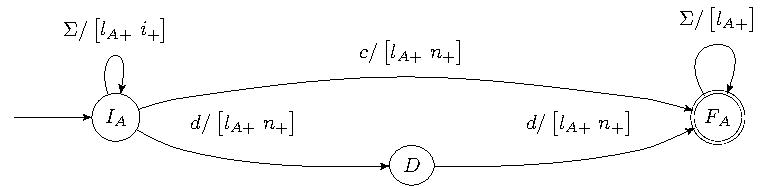
\includegraphics[scale=\autscale]{a}
    \caption{The automaton $A'$, whose Parikh registers count both the number of letters and the start ($l$) and length ($r$) of the substring matching $\Regex{c\RegexOr{}dd}$.}\label{fig:aut_a}
      %\Description[SHORT]{LONG}
  \end{subfigure}
  \begin{subfigure}[b]{0.5\textwidth}
    \centering
    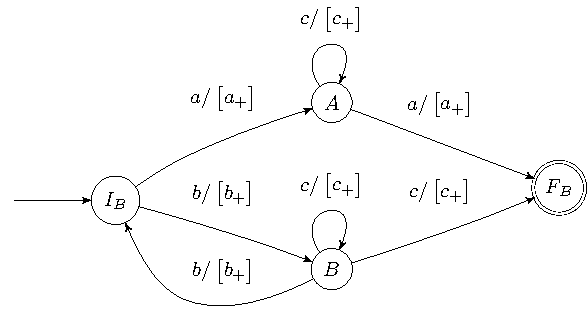
\includegraphics[scale=\autscale]{b}
    \caption{The automaton $B$, where the Parikh registers count the number of occurrences of each letter.}\label{fig:aut_b}
      %\Description[SHORT]{LONG}
  \end{subfigure}
  \caption{The collection of automata we use as running examples}\label{fig:examples}
\end{figure}


In this section we will introduce an intuition for how a string constraint problem in an automata-based solver like \OstrichPlus{} is translated to a Parikh automata intersection problem and solved efficiently using \Calculus{}. First, by a Parikh automaton we mean a standard Non-deterministic finite automaton (NFA) with a set of Parikh registers that are incremented (or decremented) at each transition. In the automata of \cref{fig:examples}, we will use the notation $a / \begin{bmatrix} x_+ \end{bmatrix}$ to mean that a transition reads an input character $a$ and increments register $x$ by one. We will omit any zero-valued increments and assume that all registers are scoped to their automaton. The increments are in reality a vector (hence the notation), but as it is mostly sparse here, we instead use the symbolic notation $\begin{bmatrix} x_{1+} \end{bmatrix}$ rather than the more cumbersome $\begin{bmatrix} 0 \\ 1 \\ 0 \\  \vdots \\ 0 \end{bmatrix}$.

Furthermore, we use $\CountOf{c}(A)$ to refer to the number of letters $c$ in $\Language(A)$, and allow this expression to be used both in linear constraints of the input language of \cref{ex:string-constraints} and in the langauge of constraints that we translate to. Where the automaton $A$ is apparent, we will omit it.

\begin{example}\label{ex:string-constraints}
    Consider the following set of string constraints:
\begin{constraints}
    \item\label{const:x-in-c-dd} $x \in \Regex{c\RegexOr{}dd}$
    \item\label{const:y-in-b} $y \in \Language(B)$, the language accepted by automaton~$B$ of \cref{fig:aut_b}.
    \item\label{const:x-substring} $x = \Substring(y, l, r)$
    \item\label{const:more-a-than-b} $\CountOf{\Char{a}}(y) > \CountOf{\Char{b}}(y)$, that is $y$ contains more letters \Char{a} than letters \Char{b}.
\end{constraints}
\end{example}

\cref{const:x-in-c-dd,const:y-in-b,const:x-substring} can be translated to the product of Parikh automata $B \times A'$, where $A'$ (\cref{fig:aut_a}) is the Parikh automata obtained by applying the encoding of $\Substring$ described in \cite{ostrich-plus}. Here follows an intuition for our method on $B \times A'$ under the global constraint \cref{const:more-a-than-b}. Note that the cost registers of \cref{fig:aut_b} are simply counting letters.

Our approach to the computation of the Parikh image (and therefore the solution to the intersection problem posed by \cref{ex:string-constraints}) consists of two applications of laziness; late computation of products of automata, and lazy enforcement of connectivity constraints. Both are in contrast to the eager approach to finding the Parikh image described in~\cite{generate-parikh-image}.

Starting with an interactive theorem prover and the goal of solving the constraint $\CountOf{\Char{a}}(B \times A') > \CountOf{\Char{b}}(B \times A')$ we associate each transition of $A'$ and $B$ with a fresh integer variable, $\TransitionVar_\Transition$, identically to \cite{generate-parikh-image}. These variables represent how many times each transition is taken. Hence, the final counter value for each automaton is the element-wise sum:
\begin{equation}
\begin{bmatrix} \CountOf{\Char{a}} \\ \CountOf{\Char{b}} \\ \CountOf{\Char{c}} \\ \CountOf{\Char{d}} \end{bmatrix} = \sum_\Transition \TransitionVar_\Transition \cdot \IncrementVec_\Transition \text{ where $\IncrementVec_\Transition$ are the increments of transition $\Transition$}.
\end{equation}


We start by adding linear constraints requiring transition variables to represent a flow through either automata by requiring that the number of incoming transitions is equal to the number of outgoing ones, and use the automated theorem prover to annotate each transition $\Transition$ with a symbolic representation of its associated integer variable:
\begin{figure}[h]
    \centering 
  \begin{subfigure}[b]{0.5\textwidth}
    \centering
    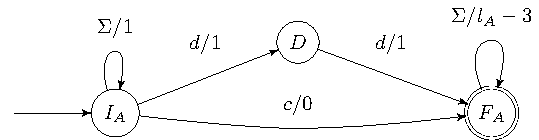
\includegraphics[scale=\autscale]{a_annotated}
    \caption{Note: unused self-loops at $I_{A'}$ and $F_{A'}$ have been pruned for readability.}\label{fig:aut_a_annotated}
      %\Description[SHORT]{LONG}
  \end{subfigure}
  \begin{subfigure}[b]{0.5\textwidth}
    \centering
    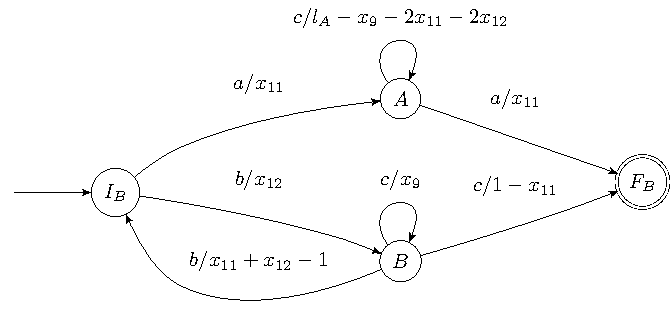
\includegraphics[scale=\autscale]{b_annotated}
    \caption{}\label{fig:aut_b_annotated}
      %\Description[SHORT]{LONG}
  \end{subfigure}
  \caption{The starting automata, without their counter increments and with their transition variables in symbolic form.}\label{fig:propagated}
\end{figure}

Note that several transitions are already marked as unuseable (have a transition value of $0$). This includes any transition for the letter $\Char{d}$, as all counter increments for that variable in $B$ is zero and hence it must also be zero in the product of both automata. By removing these transitions to obtain new automata and computing their product, we obtain the following:

\begin{figure}[h]
    \centering 
    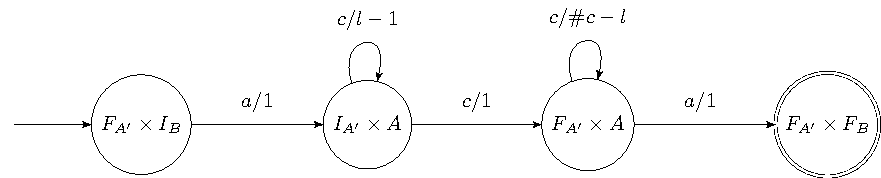
\includegraphics[scale=\autscale]{ab}
  \caption{An automaton encoding the constraint $\CountOf{\Char{a}}(B \times A') > \CountOf{\Char{b}}(B \times A')$.}\label{fig:product}
      %\Description[SHORT]{LONG}
\end{figure}

By putting off computing the product $B \times A'$ until after performing linear reasoning on the number of times each transition must be taken, we have constructed a much smaller product than we would have originally. Moreover, since this automaton is a stick, all runs through it can be described by the flow-preservation equations described above without the need for costly connectivity-enforcing constraints as in~\cite{generate-parikh-image}. This illustrates the advantage of our second laziness: deferred enforcement of connectivity constraints.